% Generated by Look@NanoSIMS (12-Nov-2011 13:21:28)
% /home/lpolerec/nanosimsdata/test_data/Ecoli_Azo_Gam42a_5/
\documentclass[12pt,a4paper]{article}
\usepackage{graphicx}
\usepackage[left=1in,right=1in,top=1in,bottom=1in]{geometry}
\begin{document}
\begin{center}
\begin{tabular}{cc}
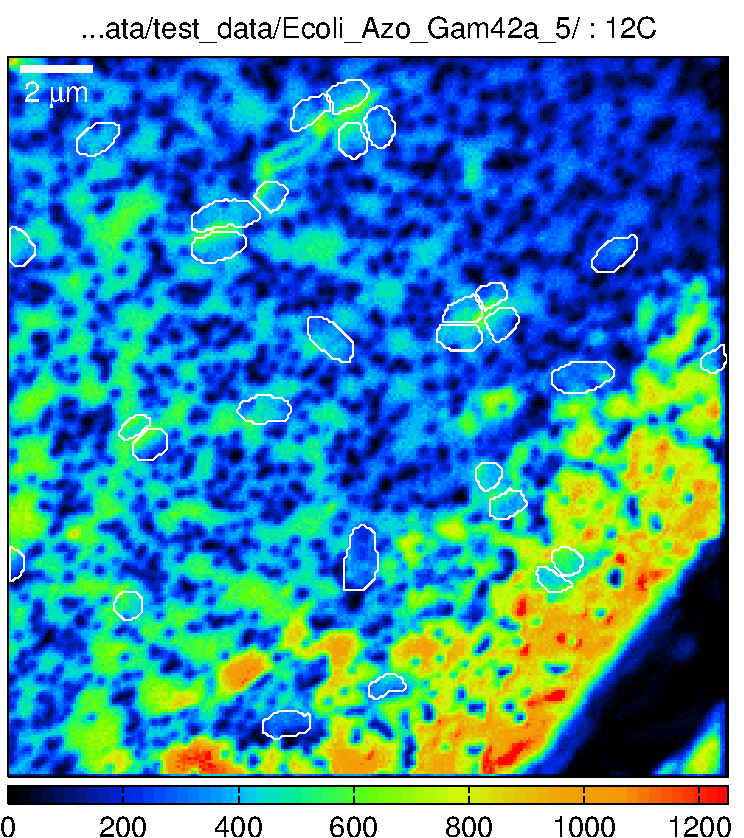
\includegraphics[width=0.42\textwidth]{pdf/12C} & 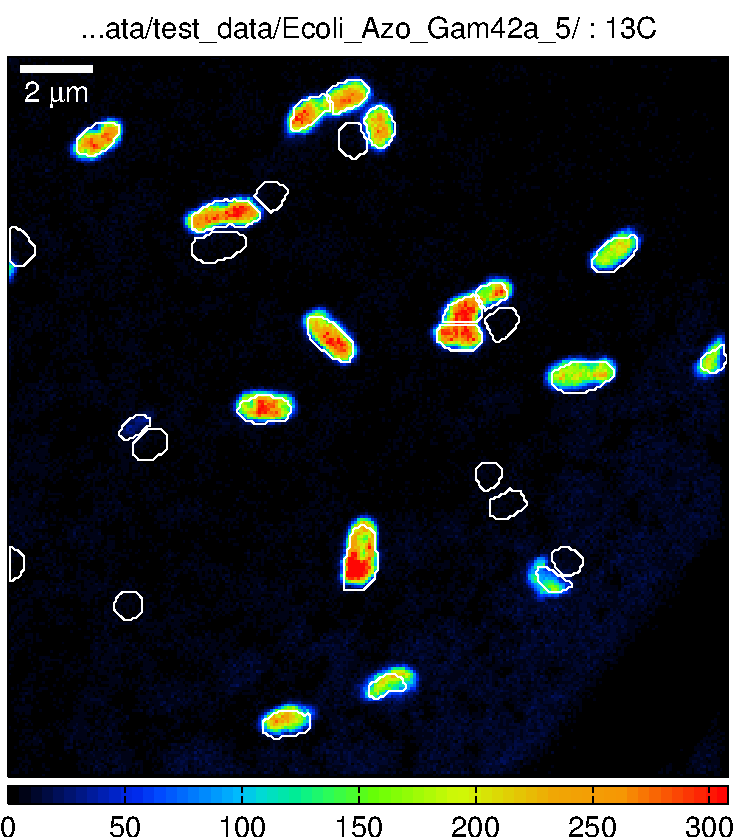
\includegraphics[width=0.42\textwidth]{pdf/13C} \\
\end{tabular}
\begin{tabular}{cc}
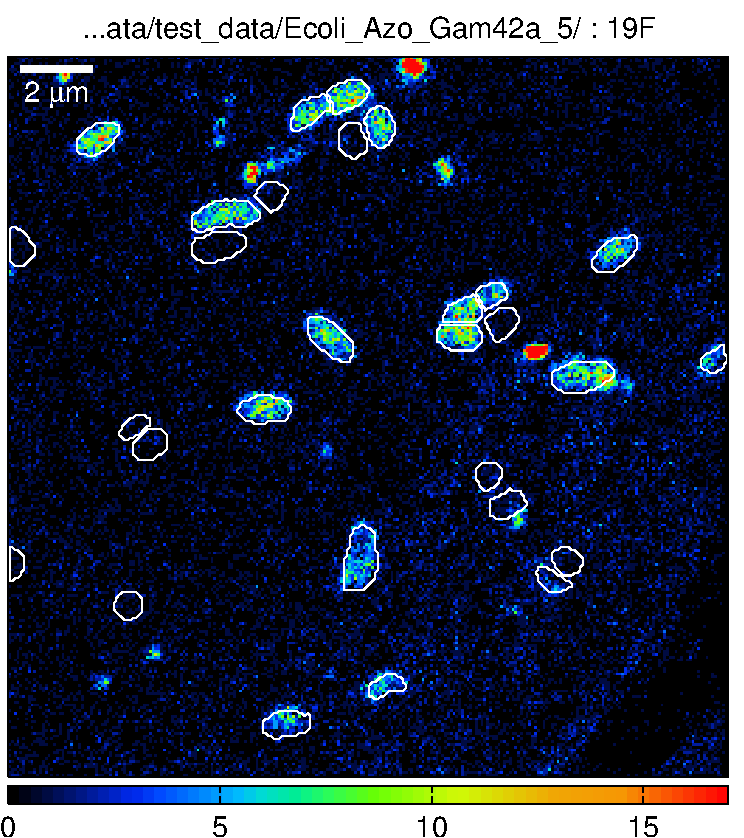
\includegraphics[width=0.42\textwidth]{pdf/19F} & 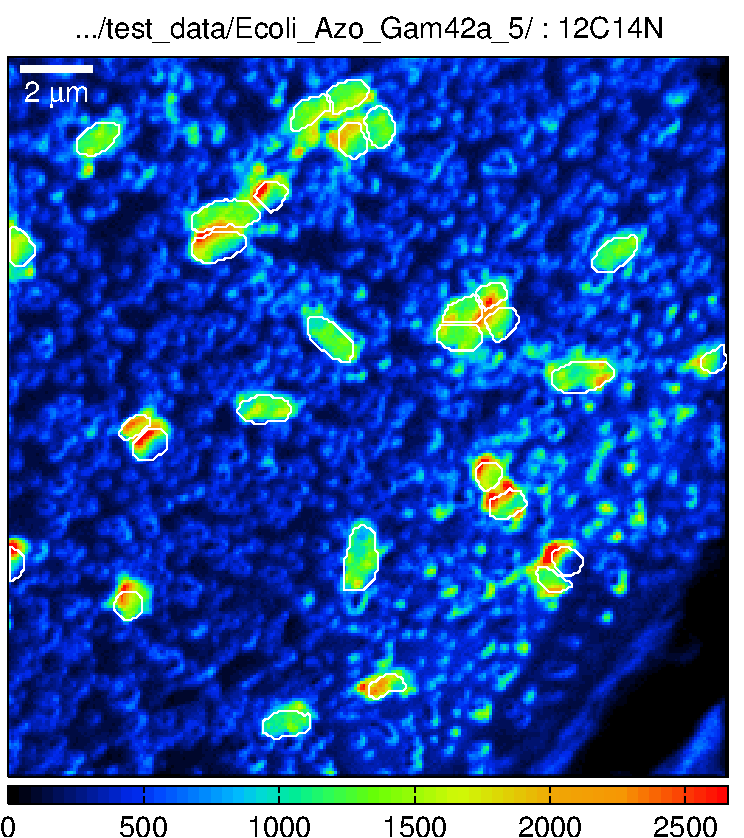
\includegraphics[width=0.42\textwidth]{pdf/12C14N} \\
\end{tabular}
\begin{tabular}{cc}
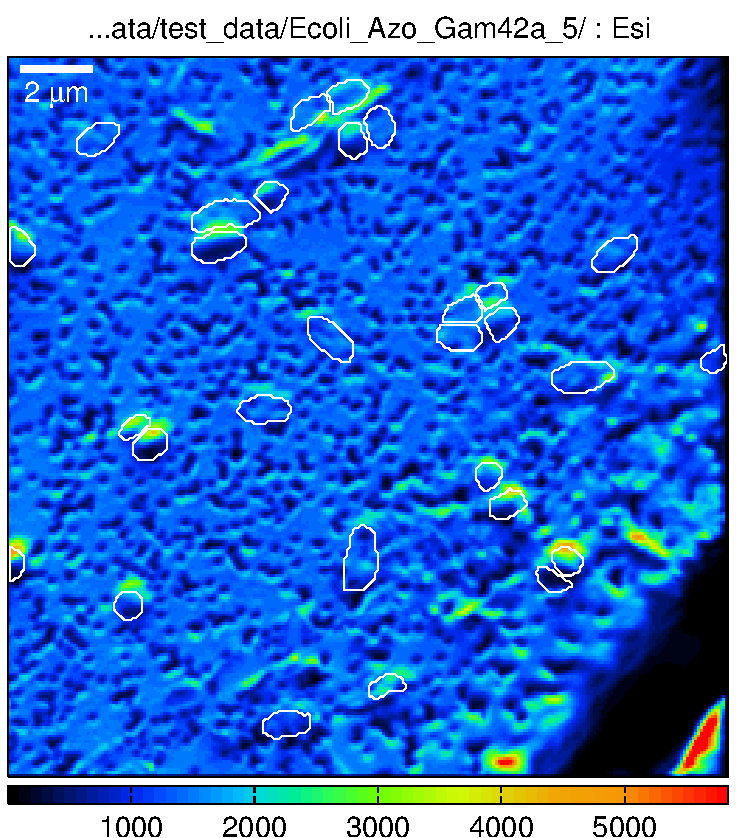
\includegraphics[width=0.42\textwidth]{pdf/Esi} & 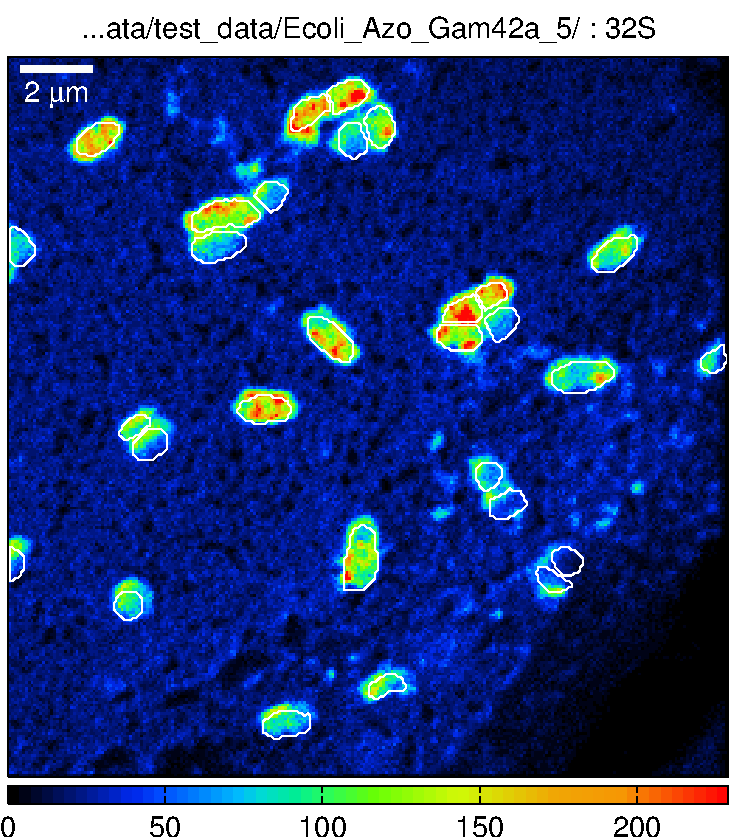
\includegraphics[width=0.42\textwidth]{pdf/32S} \\
\end{tabular}
\begin{tabular}{cc}
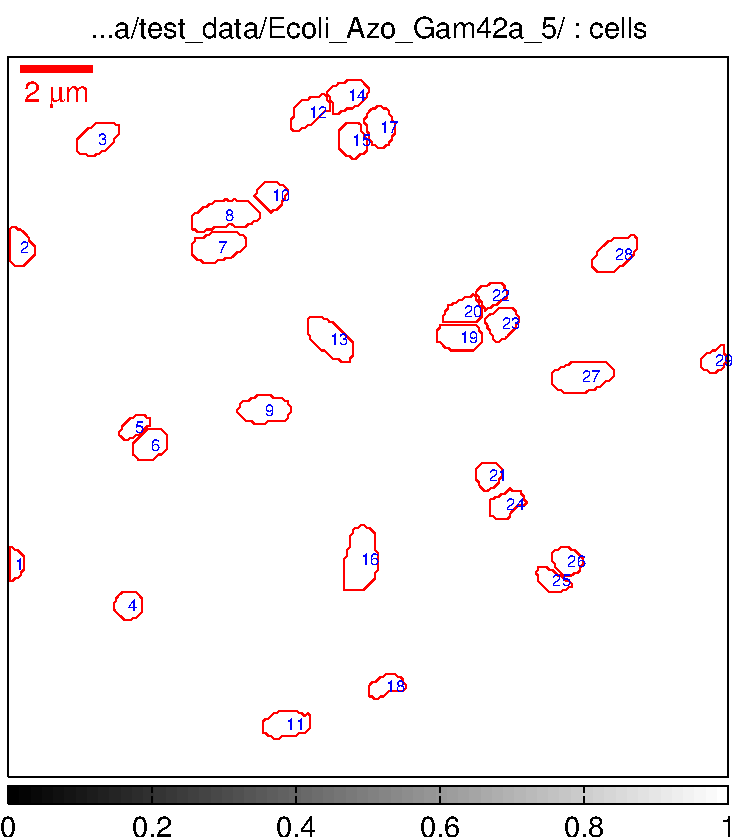
\includegraphics[width=0.42\textwidth]{pdf/cells} & 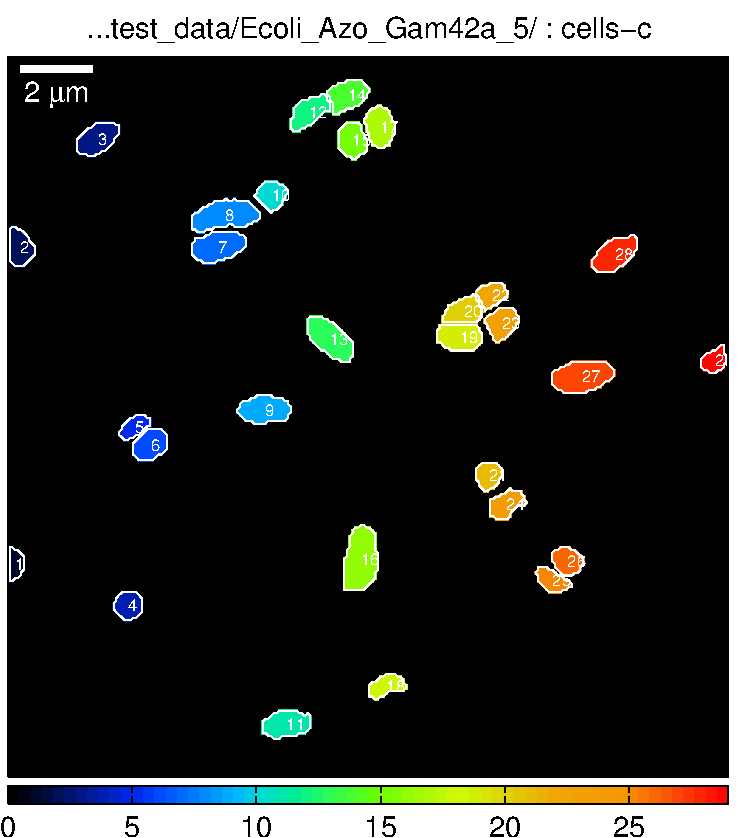
\includegraphics[width=0.42\textwidth]{pdf/cells-c} \\
\end{tabular}
\begin{tabular}{cc}
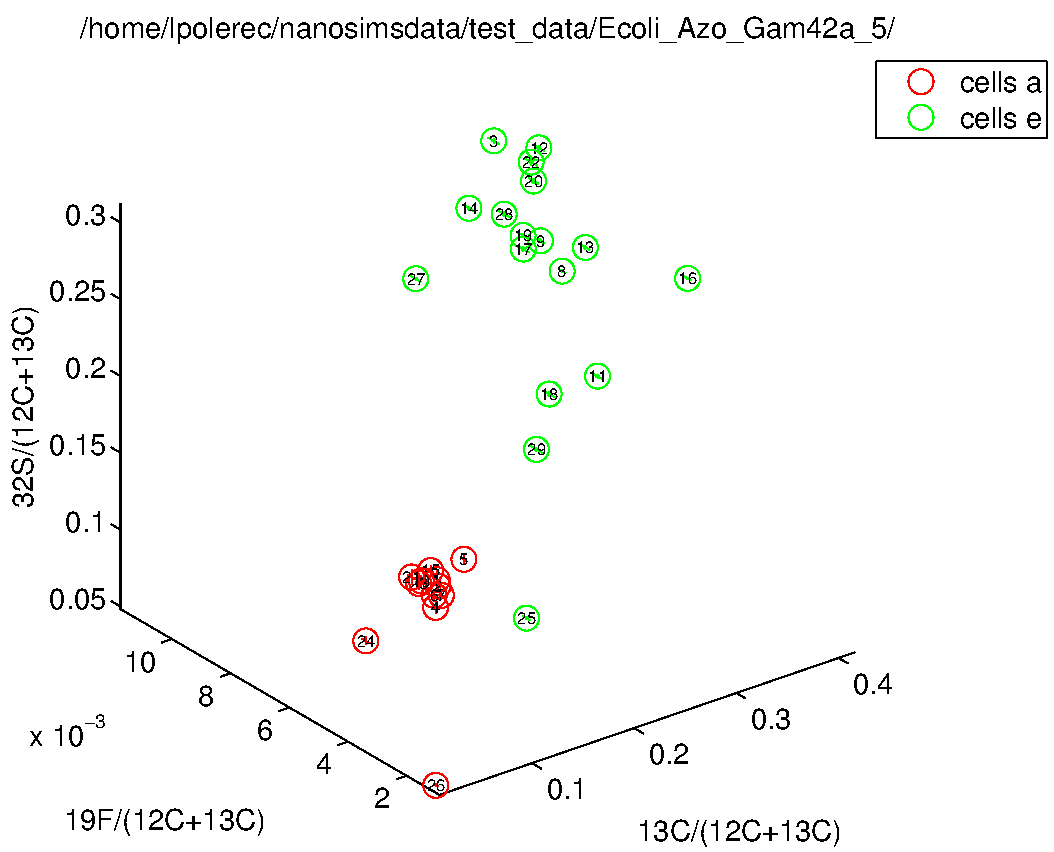
\includegraphics[width=0.42\textwidth]{pdf/13C-(12C+13C)-vs-19F-(12C+13C)-vs-32S-(12C+13C)} & 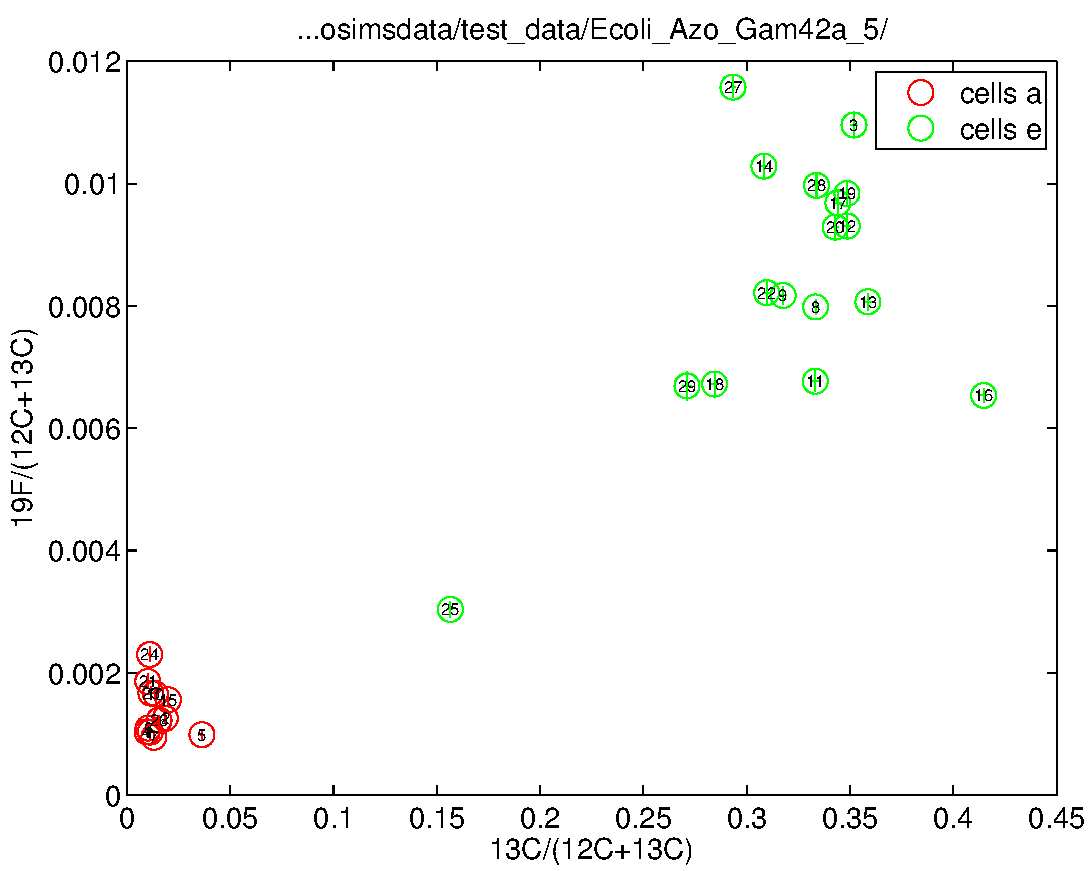
\includegraphics[width=0.42\textwidth]{pdf/13C-(12C+13C)-vs-19F-(12C+13C)} \\
\end{tabular}
\begin{tabular}{cc}
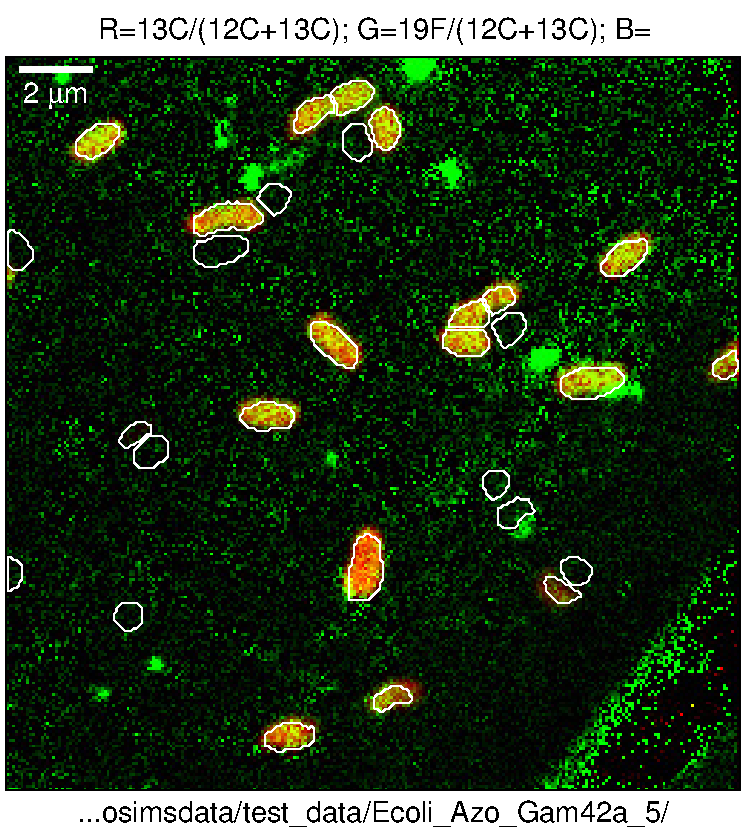
\includegraphics[width=0.42\textwidth]{pdf/13C-12C+13C-vs-19F-12C+13C-rgb} & 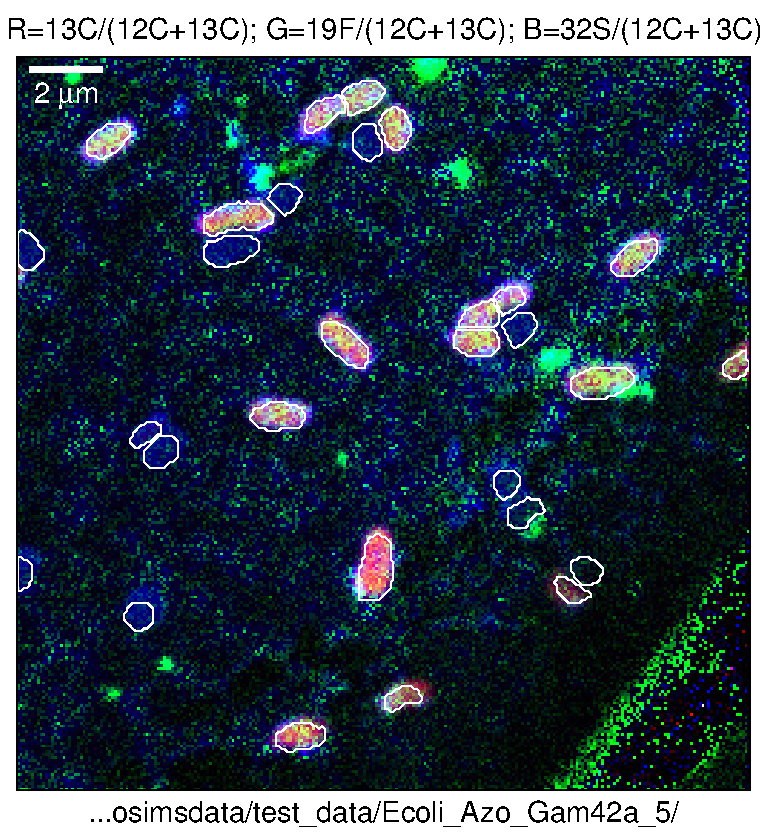
\includegraphics[width=0.42\textwidth]{pdf/13C-12C+13C-vs-19F-12C+13C-vs-32S-12C+13C-rgb} \\
\end{tabular}
\end{center}
\end{document}